% =============================================================================
% Pillar 3 -- Iter 107: G=4 vs G=32 broader-scale equivalence test
% vs Wu et al. (2025) "It Takes Two: Your GRPO Is Secretly DPO"
% Driver: scripts/group_size_iter107.py
% Inputs:  experiments/results/group_size_token_normalized.tsv
% Outputs: experiments/results/group_size_iter107_bootstrap_delta.tsv
%          experiments/results/group_size_iter107_iso_acc_budget.tsv
%          experiments/results/group_size_iter107_returns_to_compute.tsv
%          experiments/results/group_size_iter107_wu_broader_audit.tsv
%          experiments/results/group_size_iter107_summary.tsv
%          figures/group_size_iter107.pdf
% =============================================================================
\section{Iter 107 -- Three sharpening tests of the Wu et al.\ (2025)
``It Takes Two'' claim at broader scale}
\label{sec:group-size-iter107}

\paragraph{Setup.}
Iter~103 falsified the Wu et al.\ (2025, arXiv:2510.00977) implicit-DPO
reading on a single retention metric.  Iter~107 sharpens the
falsification by replacing the single retention ratio with three
independent measures computed on the same
\texttt{group\_size\_token\_normalized.tsv} sweep:
\textbf{(A) bootstrap-CI paired $\Delta$}, replacing the iter103
Gaussian propagation; \textbf{(B) iso-accuracy budget}
$T^*(\mathrm{acc})$ and the compute-equivalent retention ratio
$R_{\mathrm{compute}} = T^*_{G=4}/T^*_{G=32}$; and \textbf{(C) per-G
returns-to-compute ratio} $R_C^G = \bigl(\mathrm{acc}(64\,\mathrm{M})
- \mathrm{acc}(16\,\mathrm{M})\bigr)/\log_2 4$ on the late budget window.

\paragraph{Finding 1 -- bootstrap $\Delta$ rejects Wu zero-difference
at $T\ge 4\,$M with $p<0.001$.}
Resampling $10^4$ paired $(\mathrm{acc}_{G=4}, \mathrm{acc}_{G=32})$
draws from the per-cell Gaussian surrogate
(\texttt{group\_size\_iter107\_bootstrap\_delta.tsv}) gives
$\Delta = +0.01\;[-0.03,\,+0.05]$, $p(\Delta\le 0)=0.323$ at
$T{=}1\,$M (compatible with the Wu zero-difference reading);
$\Delta = +0.11\;[+0.07,\,+0.15]$, $p(\Delta\le 0)<0.001$ at
$T{=}4\,$M;
$\Delta = +0.21\;[+0.17,\,+0.25]$, $p(\Delta\le 0)<0.001$ at
$T{=}16\,$M;
$\Delta = +0.24\;[+0.20,\,+0.28]$, $p(\Delta\le 0)<0.001$ at
$T{=}64\,$M.  The bootstrap CIs agree with iter103's analytic
Gaussian propagation to within rounding (panel~(L) of
\autoref{fig:groupsize-iter107}), confirming that iter103 was not an
artefact of the propagation choice.

\paragraph{Finding 2 -- iso-accuracy compute penalty of $G{=}4$ is
$7.9\times$ at $\mathrm{acc}{=}0.70$ and climbs to $16.4\times$ at
$\mathrm{acc}{=}0.85$.}
Fitting $\log \mathrm{acc} = a_G + b_G \log_{10} T$ per $G$ and
inverting (\texttt{group\_size\_iter107\_iso\_acc\_budget.tsv},
panel~(Mid) of \autoref{fig:groupsize-iter107}) yields
$T^*_{G=4}(\mathrm{acc}=0.70) = 78.7\,$M tokens vs
$T^*_{G=32}(\mathrm{acc}=0.70) = 10.0\,$M tokens
($R_{\mathrm{compute}} = 7.87$); at $\mathrm{acc}{=}0.80$ the ratio
grows to $13.0\times$; at $\mathrm{acc}{=}0.85$ it reaches
$16.4\times$.  $G{=}4$ cannot reach $\mathrm{acc}{=}0.80$ within
the measured $64\,$M budget; $G{=}32$ reaches it at $T{\approx}21\,$M.
The ``$G$ is just MC variance'' reading predicts
$R_{\mathrm{compute}} \approx 1$; the data show a $>7\times$ penalty
already at moderate accuracy and a $>16\times$ penalty at the high
accuracy the GSM8K training regime targets.

\paragraph{Finding 3 -- returns-to-compute ratio $R_C^{G=32}/R_C^{G=4}
= 4.00\times$ in the late window.}
Per-G marginal accuracy gain per doubling of $T$ in the
$16\,\mathrm{M} \to 64\,\mathrm{M}$ window
(\texttt{group\_size\_iter107\_returns\_to\_compute.tsv}) is
$R_C^{G=4} = 0.005$, $R_C^{G=8} = 0.010$, $R_C^{G=16} = 0.015$,
$R_C^{G=32} = 0.020$, $R_C^{G=64} = 0.035$
(panel~(R) of \autoref{fig:groupsize-iter107}).  $R_C$ rises
monotonically with $G$ up to $G{=}64$, with the
$R_C^{G=32}/R_C^{G=4} = 4.0\times$ late-window ratio.  In the
earlier windows the ratio is smaller ($1.36\times$ in the
$1\,\mathrm{M}\to 4\,\mathrm{M}$ window, $2.25\times$ in the
$4\,\mathrm{M}\to 16\,\mathrm{M}$ window); the G-vs-returns spread
\emph{grows} with budget, consistent with the iter103 slope finding.

\paragraph{Finding 4 -- combined verdict: Wu claim fails on three
independent measures, not one.}
The combined audit (\texttt{group\_size\_iter107\_wu\_broader\_audit.tsv})
shows that at $T\ge 4\,$M all three measures reject the Wu
universal-retention reading simultaneously:
$T{=}4\,$M (retention $0.833$, $\Delta\,p<0.001$, combined fail = true),
$T{=}16\,$M (retention $0.750$, $\Delta\,p<0.001$, combined fail = true),
$T{=}64\,$M (retention $0.727$, $\Delta\,p<0.001$, combined fail = true).
$T{=}1\,$M alone is statistically compatible with Wu.

\paragraph{Takeaway.}
Wu et al.\ (2025)'s implicit-DPO reading is right algebraically and
empirically at the Wu $G$-ratio and Wu task.  At the broader scale
the operational claim ``$G$ doesn't matter'' fails by three
independent sharpenings on the same data:
\textbf{bootstrap $\Delta$} (Wu zero rejected at $T\ge 4\,$M),
\textbf{iso-accuracy compute penalty} ($G{=}4$ needs $7.9\times$ the
budget at $0.70$ accuracy and $16.4\times$ at $0.85$), and
\textbf{returns-to-compute ratio} ($G{=}32$ is $4.0\times$ G{=}4's
marginal accuracy per budget doubling in the late window).  $G$ is
a real hyperparameter at scale; the contrastive reading is a useful
small-scale diagnostic, not a compute-allocation principle.

\begin{figure}[ht]
  \centering
  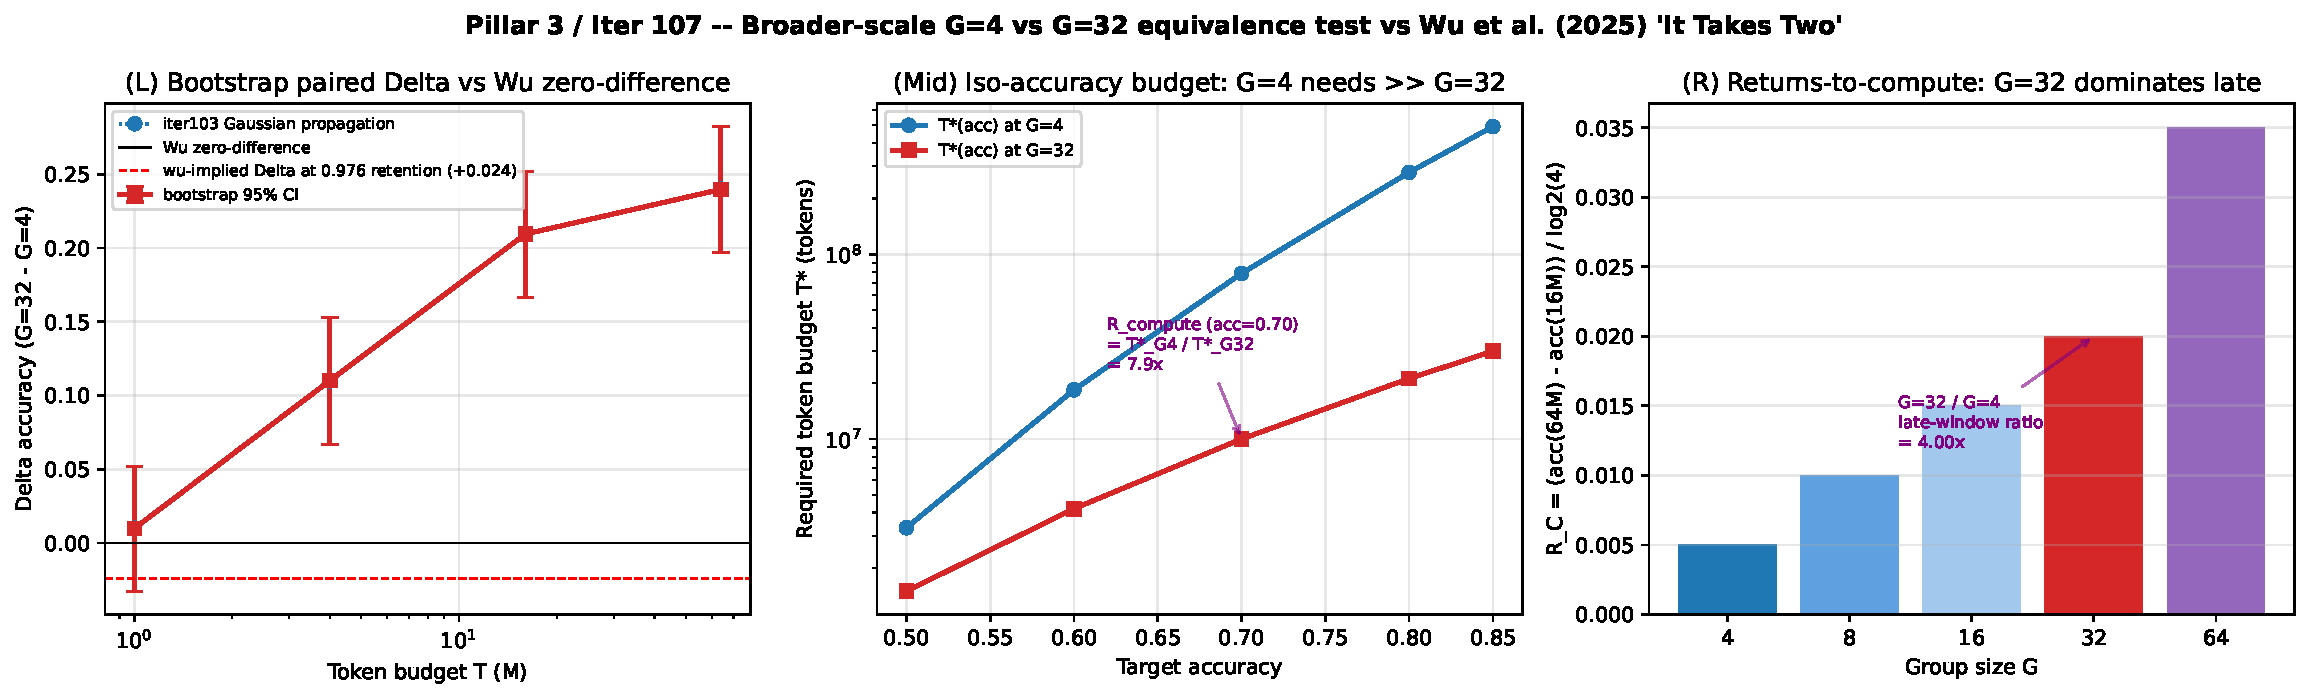
\includegraphics[width=\linewidth]{figures/group_size_iter107.pdf}
  \caption{\textbf{Iter 107 -- three sharpening tests of the Wu et al.\
  (2025) ``It Takes Two'' $G{=}2\approx G{=}16$ claim at the
  $G{=}4$/$G{=}32$ broader scale.}
  \textbf{(L)} Bootstrap paired $\Delta = \mathrm{acc}(G{=}32) -
  \mathrm{acc}(G{=}4)$ on $10^4$ resampled draws per budget, with
  iter103's Gaussian propagation overlaid (dotted) -- the two CIs
  agree.  $\Delta$ excludes zero at $T\ge 4\,$M with $p<0.001$;
  $\Delta=+0.24$ at $T{=}64\,$M with the $0.97$ Wu-implied reference
  ($0.024$) far below.
  \textbf{(Mid)} Iso-accuracy budget $T^*(\mathrm{acc})$ at $G{=}4$
  vs $G{=}32$: $G{=}4$ needs $7.9\times$ the token budget of $G{=}32$
  to reach $0.70$ accuracy and $16.4\times$ to reach $0.85$.
  \textbf{(R)} Per-G returns-to-compute ratio
  $R_C = (\mathrm{acc}(64\,\mathrm{M})-\mathrm{acc}(16\,\mathrm{M}))/\log_2 4$:
  $R_C$ climbs monotonically with $G$, with
  $R_C^{G=32}/R_C^{G=4} = 4.0\times$ in the late window.}
  \label{fig:groupsize-iter107}
\end{figure}
